\documentclass[titlepage, letterpaper, 11pt]{article}
\usepackage[letterpaper, margin=1.25in]{geometry}
\usepackage{graphicx}
\usepackage{amsmath}
\begin{document}

\title{Multi-Stage Tuned Amplifier}
\author{By: Ben Lorenzetti\\
Team Member: Francois Nyamsi}
\date{Project Start Date: January 22, 2015\\
Report Submission Date: February 8, 2015}
\maketitle

\clearpage
\mbox{}
\thispagestyle{empty}
\clearpage
\setcounter{page}{1}

\tableofcontents

\section{Objective}

To compare the operation of common-emitter and common-base tuned
amplifier stages, and to design and characterize a multi-stage,
high-gain IF amplifier for 10 MHz operation with 50$\Omega$ input and
output impedances.

\clearpage
\section{Principles of Operation}

Tuned amplifiers are critical for electronic communications because
they increase the power of desired signal but reject other frequencies
as noise. At 10 MHz, a tuned amplifier could be used with an antenna
to recieve HF amateur radio from the other side of the world
\footnote{10 MHz waves can traverse the curve of the earth because
they get reflected by charged particles in the ionosphere, called
ionospheric skip propagation.},
or could be used in a computer to recieve 10Base-T ethernet.

There are three possible circuit configurations for bipolar junction
transistors (BJT) biased in forward-active mode, based on
which terminals are used for input, output, and common reference.

\begin{figure}[ht]
	\centering
	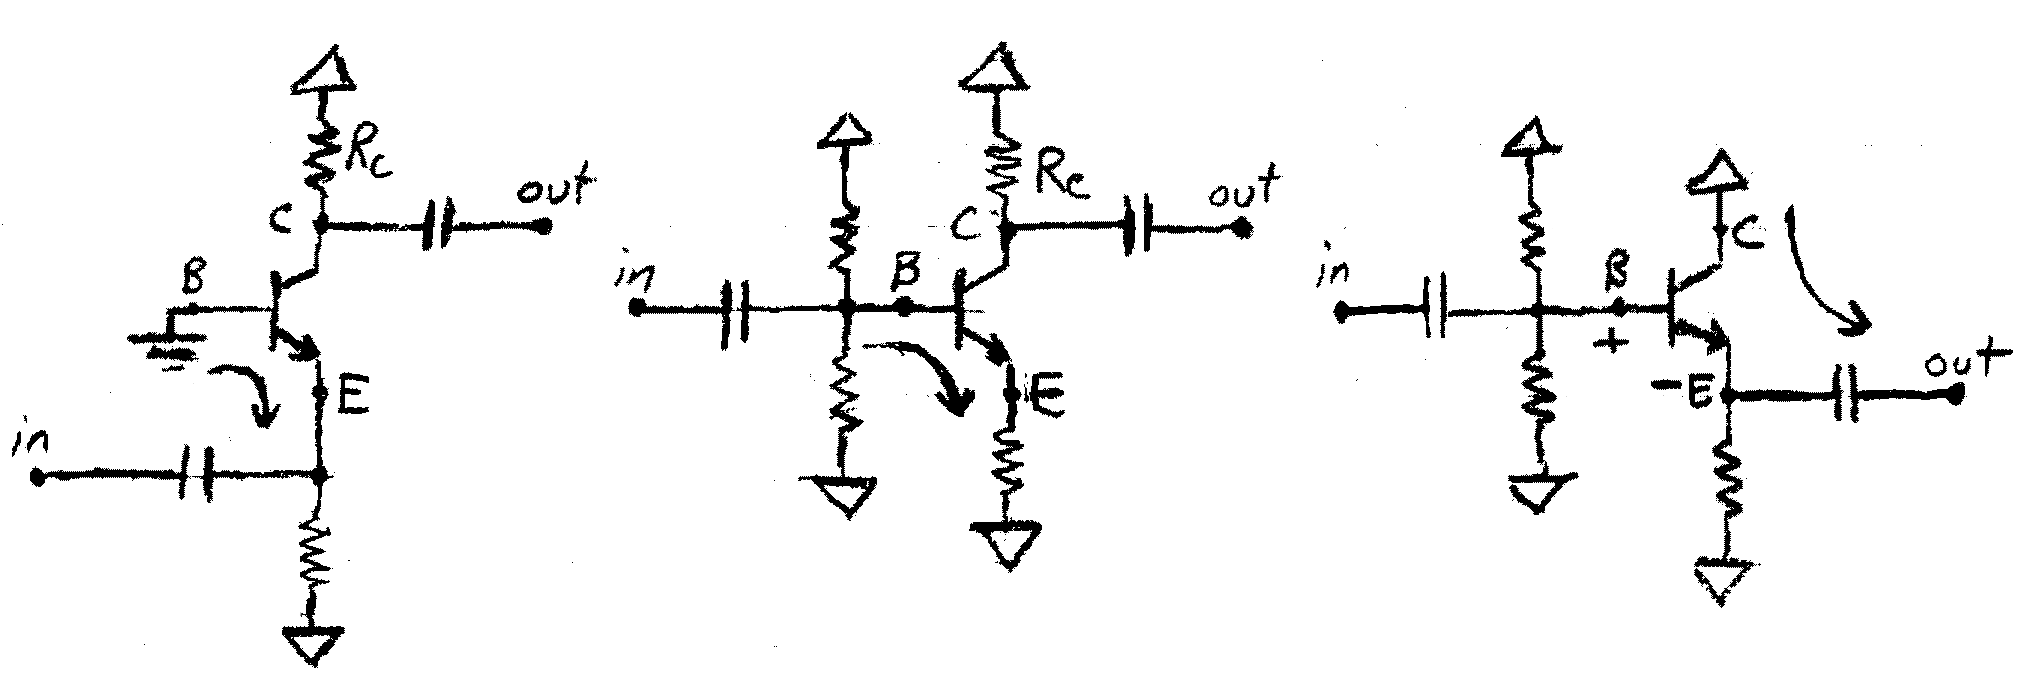
\includegraphics[width=0.75\textwidth]
		{figures/BJTforwardBiasConfigurations.png}
	\caption{
		Common-base (left), common-emitter (middle), and
		common-collector (right) configurations for BJT
		amplifiers.
	}
	\label{BJTforwardBiasConfigurations}
\end{figure}

Each configuration has its tradeoffs. The common-base (CB) configuration is
a good current buffer, with $A_{i}\approx1$ and low input impedance.
The common-emitter (CE) configuration offers the best overall power gain,
but $A_{v}$ and $A_{i}$ may vary with loadings. The common-collector
configuration is a good voltage buffer 
($A_{v}\approx1$) with low output impedance.

The three configurations can be cascaded together to gain the benefits
of each. If cascaded in the order shown in figure 
\ref{BJTforwardBiasConfigurations}, from left-to-right, the resulting
3-stage broadband amplifier would have low input impedance, good power
gain, and minimal output impedance.

A slight modification to the CE and CB configurations in figure
\ref{BJTforwardBiasConfigurations} can apply a filter to the broadband
amplifier; tuning the gain to a narrow frequency set by a tank circuit. 

Because BJTs are minority carrier devices, they act as current amplifiers
without being strongly affected by voltage. For the two configurations
where the output is at the collector (CB and CE), the BJT acts like a
dependent current source feeding the output load and the biasing
resistance $R_{C}$. As a result, the voltage gain for these
configurations is determined primarily by how difficult it is for
the collector current to reach ground; $A_{v}\propto R_{C}||R_{L}$.

One can take advantage of the collector current's obstinance
by replacing $R_{C}$ with an impedance that varies with frequency.
Using an inductor and a capacitor in parallel provides a short circuit
to ground for both DC and high frequency currents. Additionally, at the
LC circuit's resonant frequency, the net impedance $\rightarrow \infty$
due to power oscillating between the two.
\footnote{For this reason, an $L||C$ circuit is called a tank circuit.}
The result is a narrow bandpass filter at the resonant frequency, 
where $Z_{C}\rightarrow \infty$.

\section{Theory}

\subsection{Common-Base Broadband Amplifier}

The basic circuit for an single stage, common-base (CB) amplifier is
shown in figure \ref{commonBaseAmplifier}. The base terminal is
grounded and the input signal passes through the BJT from emitter
to collector. In this configuration, the BJT acts like a current
buffer, where the input current is repeated at the output regardless
of the load. 

\begin{figure}[ht]
	\centering
	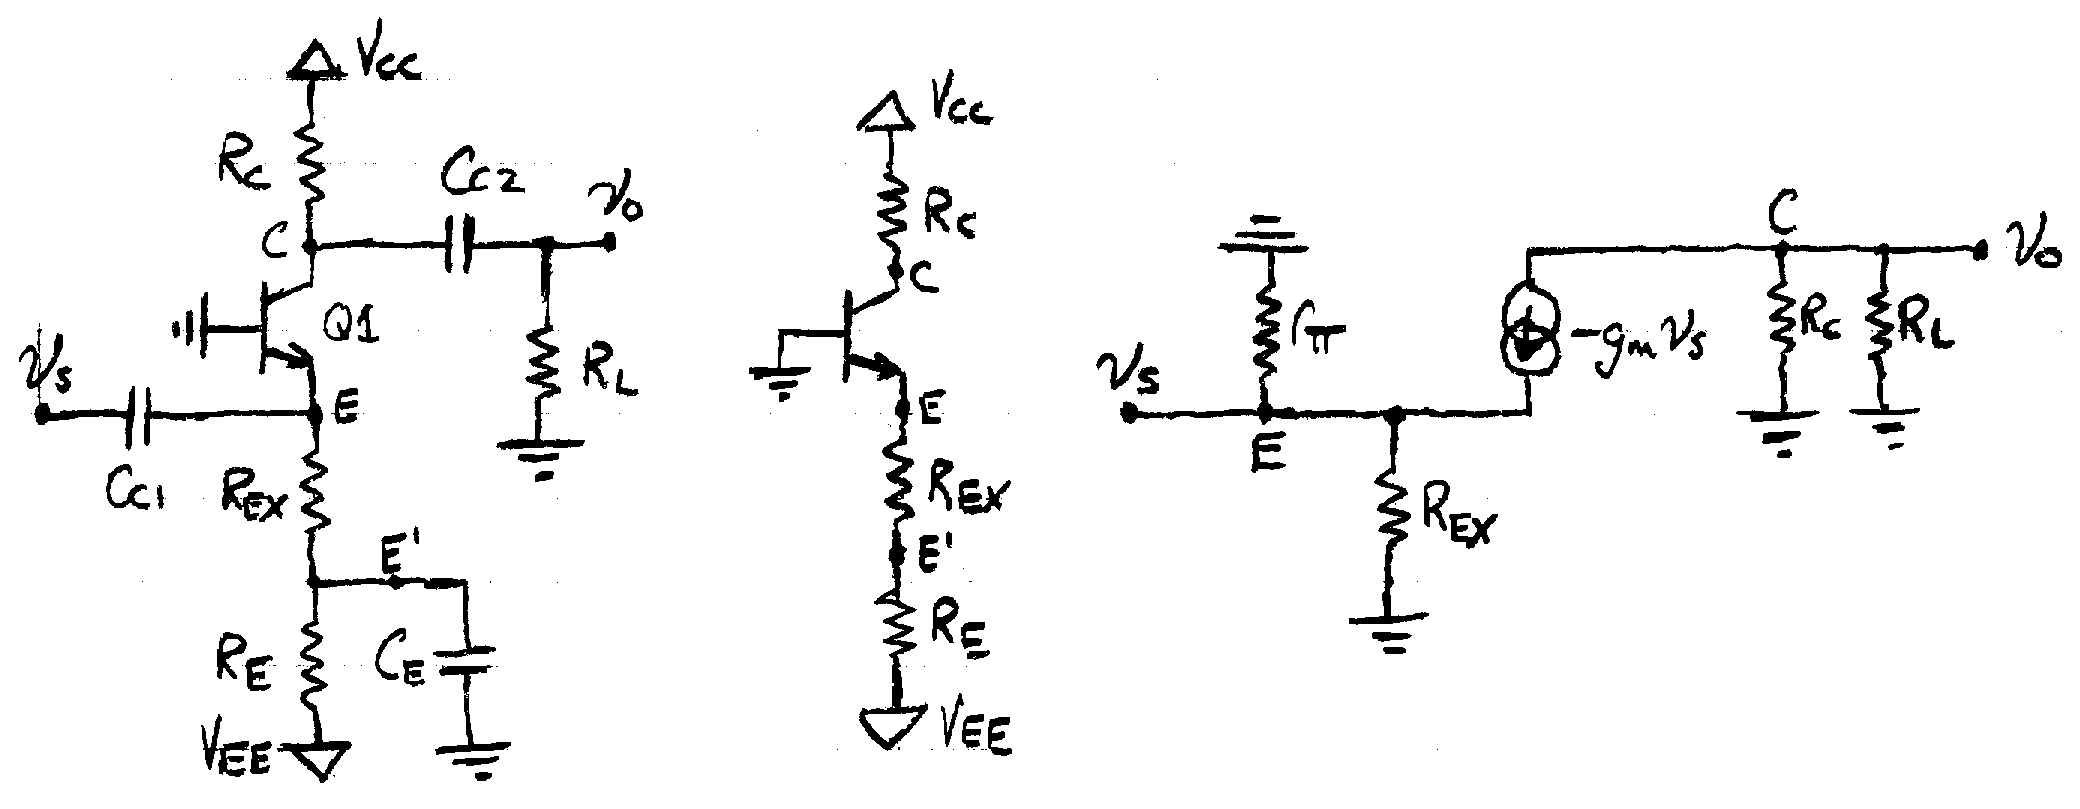
\includegraphics[width=\textwidth]
		{figures/commonBaseAmplifier.png}
	\caption{
		Basic circuit for a common-base broadband amplifier
		(left), its DC large signal (middle) equivalent, and
		AC small signal equivalent (right).
	}
	\label{commonBaseAmplifier}
\end{figure}

Two DC power rails are needed to bias the BJT in forward-active mode.
A positive supply holds the collector reverse biased
relative to the base which, at ground, is forward biased relative
to the negative supplied emitter. Quiescent point analysis of the
common-base is easy because the voltage is pinned at every node.

\begin{equation}
I_{EQ}=\frac{-V_{BE(on)}-V_{EE}}{R_{E}+R_{EX}}
\end{equation}

\begin{equation}
r_{\pi}=\frac{V_{th}}{I_{BQ}}
=\frac{V_{th}(\beta+1)(R_{E}+R_{EX})}{-V_{BE(on)}-V_{EE}}
\label{commonBaseRpi}
\end{equation}

\begin{equation}
g_{m}=\frac{\beta}{r_{\pi}}
=\frac{\alpha(-V_{BE(on)}-V_{EE})}{V_{th}(R_{E}+R_{EX})}
\end{equation}

The hybrid-$\pi$ model for small signal AC modeling is shown in the
right pane of figure \ref{commonBaseAmplifier}. Applying Kirchoff's
current law at node E can be used to find the input resistance.

\begin{equation*}
\textrm{KCL @ E:}\qquad
i_{S}-\frac{v_{s}}{r_{\pi}}-\frac{v_{s}}{R_{EX}}-g_{m}v_{s}=0
\end{equation*}

\begin{equation*}
i_{s}=v_{s} \left[ \frac{1}{R_{\pi}}+\frac{1}{R_{EX}}+g_{m} \right]
\end{equation*}

\begin{equation*}
i_{s}=v_{s} \left[
\frac{R_{EX}+r_{\pi}+g_{m}r_{\pi}R_{EX}}
{r_{\pi}R_{EX}} \right]
\end{equation*}

\begin{equation*}
\frac{v_{s}}{i_{s}}
=\frac{r_{\pi}R_{EX}}{R_{EX}+r_{\pi}+g_{m}r_{\pi}R_{EX}}
\end{equation*}

\begin{equation}
R_{in}=\frac{R_{EX}}{1+\frac{(\beta+1)R_{EX}}{r_{\pi}}}
\label{commonBaseRin}
\end{equation}

Applying KCL at the collector can be used to calculate the voltage
gain of a single common-base stage.

\begin{equation*}
-g_{m}v_{s}+\frac{v_{o}}{R_{L}}+\frac{v_{o}}{R_{C}}=0
\end{equation*}

\begin{equation*}
v_{o}\left[\frac{R_{L}+R_{C}}{R_{L}R_{C}}\right]=g_{m}v_{s}
\end{equation*}

\begin{equation}
A_{v}=\frac{g_{m}R_{L}R_{C}}{R_{L}+R_{C}}
\end{equation}

\section{Design and Simulation}

\subsection{Specifications}

\subsection{Tank Circuits}

\subsection{Common-Base Stage}

The first stage must be a common-base amplifier in order to achieve
low input resistance. The two resistors $R_{EX}$ and $R_{E1}$ must be
chosen to achieve desirable input resistance and voltage gain.

(circuit diagram for common-base stage here.)

It is clear that $R_{EX}$ is strongly related to $R_{in}$ from
equation \ref{commonBaseRin}. Substituting equation
\ref{commonBaseRpi} for $r_{\pi}$ into equation \ref{commonBaseRin}
yields

\begin{equation*}
R_{in}=\frac{R_{EX}}
{1+R_{EX}\left(\frac{-V_{BE(on)}-V_{EE}}{V_{th}}\right)/(R_{E1}+R_{EX})}
\end{equation*}

Using the specified value for $V_{EE}$, the standard $0.7V$ for
$V_{BE(on)}$, and the assumption that $R_{EX}<<R_{E1}$, then

\begin{equation}
R_{in}\approx\frac{R_{EX}}{1+\frac{436R_{EX}}{R_{E1}}}
\end{equation}

But should be the value of $R_{E1}$?

\end{document}
